\documentclass[compress]{beamer}
\usepackage[brazil]{babel}
\usepackage[latin1]{inputenc}
\usepackage{amsmath}
\usepackage{graphicx}
\usepackage{listings}

%%%%%%%%%%%%%%%%%%%%%%%%%%%%%
% C O N F I G U R A � � E S %
%%%%%%%%%%%%%%%%%%%%%%%%%%%%%
\pdfpageattr {/Group << /S /Transparency /I true /CS /DeviceRGB>>}

\definecolor{listinggray}{gray}{0.9}
\definecolor{lbcolor}{rgb}{1,1,1}

\lstset{
	backgroundcolor=\color{lbcolor},
	tabsize=4,
	rulecolor=,
	language=matlab,
    basicstyle=\tiny,
    upquote=true,
    aboveskip={1.5\baselineskip},
    columns=fixed,
    showstringspaces=false,
    extendedchars=true,
    breaklines=true,
    prebreak = \raisebox{0ex}[0ex][0ex]{\ensuremath{\hookleftarrow}},
    frame=single,
    showtabs=false,
    showspaces=false,
    showstringspaces=false,
    identifierstyle=\ttfamily,
}

\renewcommand{\lstlistingname}{C�digo}
\renewcommand{\lstlistlistingname}{Lista de C�digos}

\usetheme{Ilmenau}
%vinho
%\usecolortheme[RGB={75,11,31}]{structure}
%verde
%\usecolortheme[RGB={35,75,11}]{structure}
%azul
\usecolortheme[RGB={149,188,44}]{structure}
\setbeamercovered{transparent}
\setbeamertemplate{blocks}[rounded][shadow=true]
\setlength{\tabcolsep}{1mm}
%\setbeamertemplate{footline}[frame number]
\setbeamertemplate{navigation symbols}{}
\setbeamertemplate{headline}[default]
\setbeamertemplate{footline}[default]
\setbeamertemplate{footline}{\hspace*{.5cm}\scriptsize{\hfill\vspace*{0.3cm}\insertframenumber\hspace*{.5cm}}}

\newenvironment{changemargin}[2]{%
  \begin{list}{}{%
    \setlength{\topsep}{0pt}%
    \setlength{\leftmargin}{#1}%
    \setlength{\rightmargin}{#2}%
    \setlength{\listparindent}{\parindent}%
    \setlength{\itemindent}{\parindent}%
    \setlength{\parsep}{\parskip}%
  }%
  \item[]}{\end{list}}

%%%%%%%%%%%
% C A P A %
%%%%%%%%%%%

%\title{T�cnicas de Planejamento para Gera��o de Planos de Execu��o em um Sistema Gerenciador de Fluxos de Trabalho Cient�fico}

\title{SERVLETS E JSP (JEE) - Servlets}

\author{Diogo Cezar Teixeira Batista \\
       {\footnotesize\ttfamily diogo@diogocezar.com.br} \\
       {\footnotesize\ttfamily http://www.diogocezar.com}
}

\institute{\large Universidade Tecnol�gica Federal do Paran� - UTFPR}

\date{Corn�lio Proc�pio - 2012}

\begin{document}

% %%%%%%%%%%%%%%%%%%%%%%%%%%%%%%
% S L I D E S  I N I C I A I S %
%%%%%%%%%%%%%%%%%%%%%%%%%%%%%%%%

\begin{frame}
    \titlepage
\end{frame}


%%%%%%%%%%%%%%%%%%%
% C O N T E � D O %
%%%%%%%%%%%%%%%%%%%

\section[Servlets]{Servlets}

\begin{frame}[c,allowframebreaks,fragile]
    \frametitle{Servlets}
    \begin{itemize}
      \item O que � Servlet?
      \begin{itemize}
	\item � a base do desenvolvimento de aplicativos java
baseados na \textit{web};
	\item de uma maneira simples, pode ser entendida como
uma classe que � automaticamente carregada na
mem�ria e posteriormente executada por um
servidor \textit{web} especial;
      \end{itemize}
      
      \framebreak
      
      \item o servidor \textit{web} � chamado de \textit{container},
escolhas comuns entre \textit{conteiners} est�o:

      \begin{itemize}
	\item Tomcat \\ \url{http://jakarta.apache.org/tomcat/}
	\item JBoss \\ \url{http://www.jboss.org/products/index}
	\item Websphere \\ \url{http://www-306.ibm.com/software/websphere/}
      \end{itemize}
      
      \framebreak
      
      \item arquitetura servlet:
      
      \begin{itemize}
	\item o pacote \texttt{javax.servlet} prov� as classes e interfaces
para o desenvolvimento de \textit{servlets};
	\item a principal abstra��o no pacote \textit{Servlet} � a interface
\textit{Servlet}.
	\item todas as \textit{servlets} implementam esta
interface;
	\item utiliza��o indireta da interface \textit{Servlet};
	\item o mais comum � a heran�a da classe \texttt{HttpServlet},
que por sua vez implementa a interface \textit{Servlet};
	\item a interface \textit{Servlet} declara, mas n�o implementa, m�todos
de gerenciamento e comunica��o com os clientes;
      \end{itemize}
      
      \framebreak
      
      \item intera��o com o cliente:
      
      \begin{itemize}
	\item quando um \textit{servlet} aceita uma chamada de um cliente, ele
recebe dois objetos:
	\begin{itemize}
	  \item um \texttt{ServletRequest} , que encapsula a comunica��o entre o
cliente e o servidor;
	  \item um \texttt{ServletResponse} , que encapsula a comunica��o entre
o servidor e o cliente;
	\end{itemize}
	\item \texttt{ServletRequest} and \texttt{ServletResponse} s�o
interfaces definidas pelo pacote javax.servlet.
      \end{itemize}
      
      \framebreak
      
      \item a interface \texttt{ServletRequest}
      
      \begin{itemize}
	\item a interface \texttt{ServletRequest} permite ao servlet ter
acesso a:
	\begin{itemize}
	  \item informa��es como nomes de par�metros passados pelo
cliente, o protocolo usado pelo cliente e os nomes dos
\textit{hosts} remotos que fizeram a requisi��o ao servidor;

	  \item O \textit{stream} de entrada, \texttt{ServletInputStream} .
\textit{Servlets} usam o \textit{stream} de entrada para receber os dados do
cliente, como � o caso do m�todos HTTP \texttt{POST} e \texttt{GET};
	\end{itemize}
	\item A interface \texttt{HttpServletRequest} � mais usual em
ambientes HTTP;
      \end{itemize}
      
      \framebreak
      
      \item a interface \texttt{ServletResponse}
      
      \begin{itemize}
	\item a interface \texttt{ServletResponse} permite ao
\textit{servlet} m�todos para enviar ao cliente:
	\begin{itemize}
	  \item um \textit{stream} de sa�da, \texttt{ServletOutputStream} , e um
\textit{Writer} atrav�s dos quais podem ser enviados
dados de resposta ao cliente;
	\end{itemize}
	\item A interface \texttt{HttpServletResponse} � mais
usual em ambientes HTTP.
      \end{itemize}
      
      \framebreak
      
      \item hierarquia de classes de um \textit{Servlet}
      
      \begin{figure}[htb]
	  \begin{center}
	      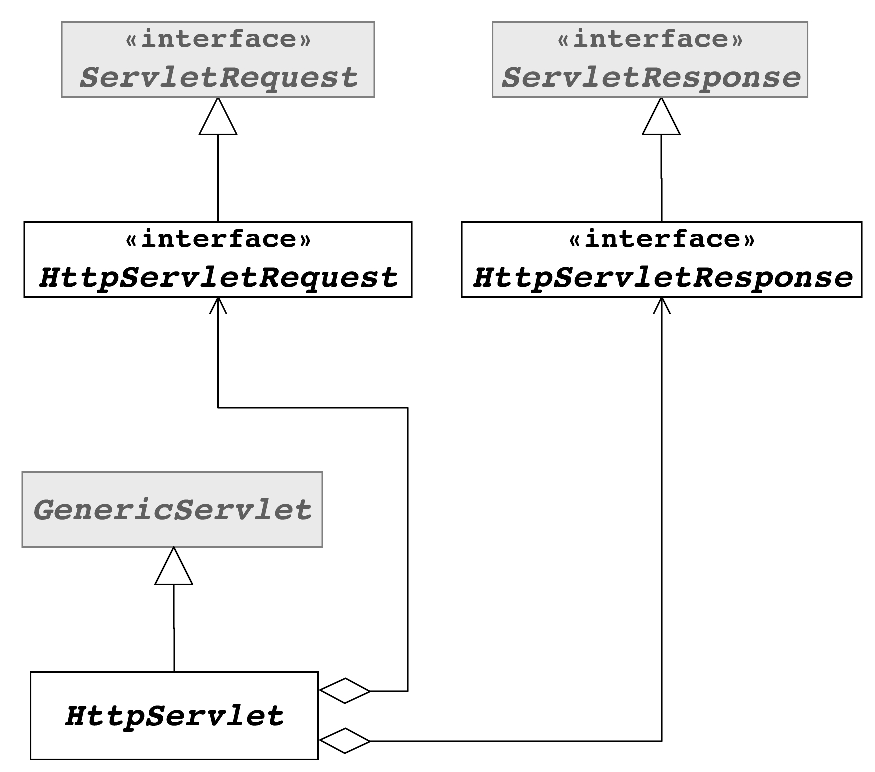
\includegraphics[width=7cm]{images/servlets-hearanca.pdf}
	  \end{center}
      \end{figure}
      
      \framebreak
      
      \item ciclo de vida de um \textit{Servlet}
      
      \begin{figure}[htb]
	  \begin{center}
	      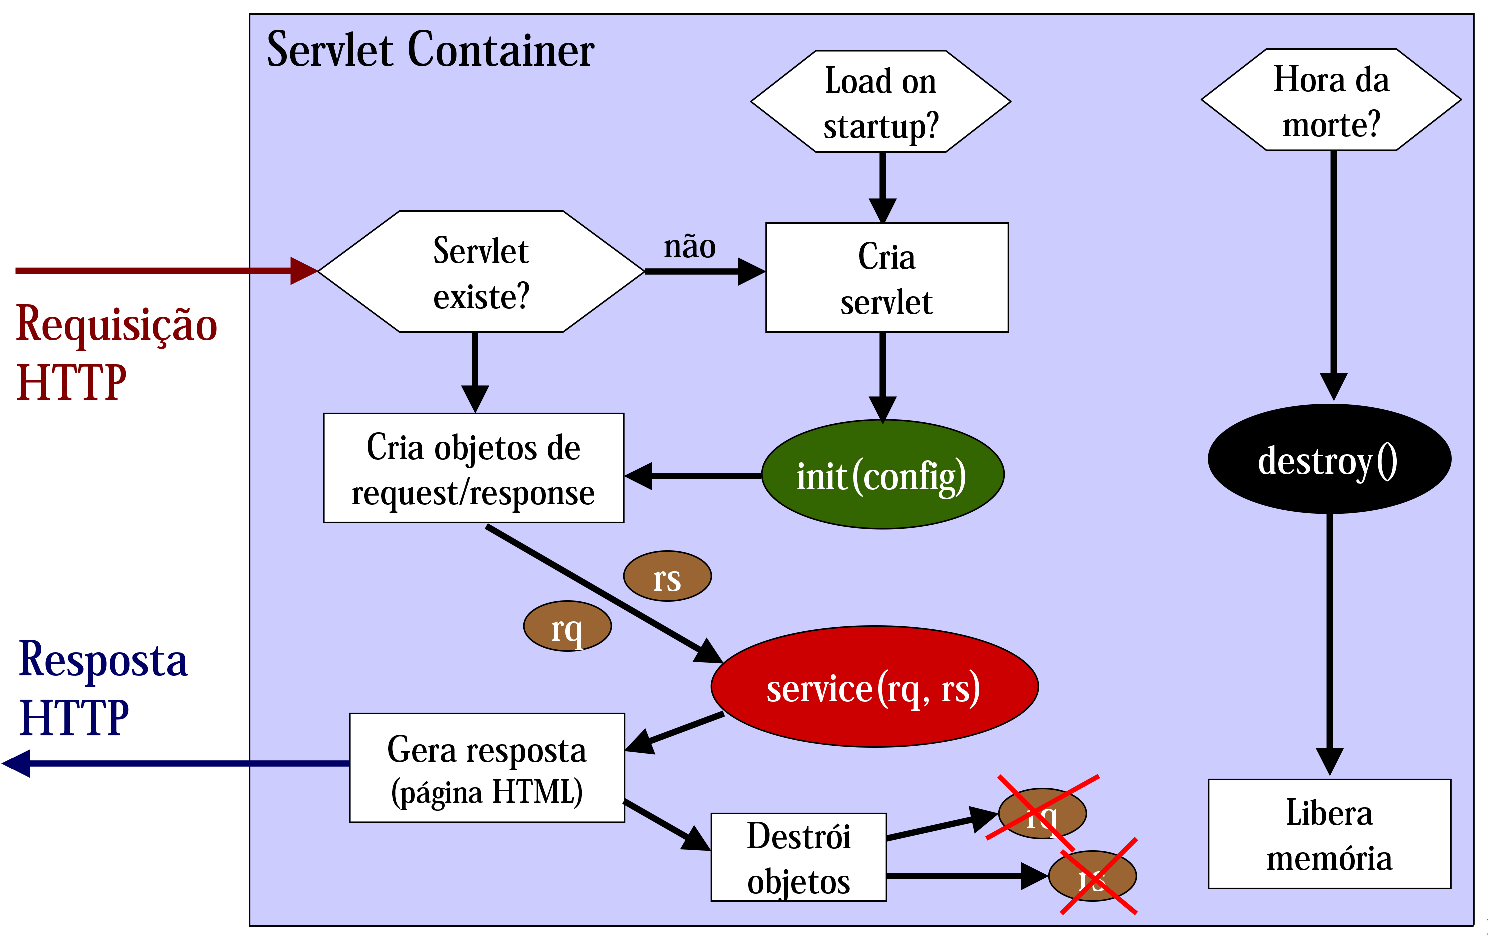
\includegraphics[width=10cm]{images/servlets-ciclo.pdf}
	  \end{center}
      \end{figure}
      
      \framebreak
      
      \item m�todo \texttt{init()} - chamado automaticamente pelo container ap�s
o carregamento da classe na mem�ria;

    \begin{center}
    \begin{minipage}{0.9\textwidth}
	\lstset{
	  frame=tb,
	  language=Java
	}
	\begin{lstlisting}
	  public void init (ServletConfig config) throws ServletException
	\end{lstlisting}
    \end{minipage}
    \end{center}
    
      \framebreak
      
      \item m�todo \texttt{service()} - � chamado pelo container logo ap�s o
m�todo \texttt{init()}, permitindo ao \textit{servlet} responder a uma
requisi��o.

    \begin{center}
    \begin{minipage}{0.9\textwidth}
	\lstset{
	  frame=tb,
	  language=Java
	}
	\begin{lstlisting}
	  public void service (servletRequest request, Servlet response
response) throws ServletException,
java.io.Exception
	\end{lstlisting}
    \end{minipage}
    \end{center}
    
      \framebreak
      
      \item m�todo \texttt{destroy()} - � chamado pelo container antes de
remover a \textit{servlet} da mem�ria;

      \framebreak
      
      \item como o \textit{servlet} implementa \textit{doGet()} e
\textit{doPost()}:

    \begin{center}
    \begin{minipage}{0.9\textwidth}
	\lstset{
	  frame=tb,
	  language=Java,
	  caption=implementado GET e POST
	}
	\begin{lstlisting}
	  public class ServletWeb extends HttpServlet {
	    public void doGet (HttpServletRequest request,
	    HttpServletResponse response) {
	      processar(request, response);
	    }
	    public void doPost (HttpServletRequest request,
	    HttpServletResponse response) {
	      processar(request, response);
	    }
	    public void processar(HttpServletRequest request,
	    HttpServletResponse response) {
	      ...
	    }
	  }
	\end{lstlisting}
    \end{minipage}
    \end{center}
    
    \framebreak
    
    \item como ler par�metros de requisi��o:
    
    \begin{itemize}
      \item formul�rios HTML codificam o texto ao enviar os dados
automaticamente;
      \item seja o m�todo POST ou GET, os valores dos par�metros
podem ser recuperados pelo m�todo \texttt{getParameter()} de
\textit{ServletRequest}, que recebe seu nome;

    \begin{center}
    \begin{minipage}{0.9\textwidth}
	\lstset{
	  frame=tb,
	  language=Java
	}
	\begin{lstlisting}
	  String parametro = request.getParameter("nome");
	\end{lstlisting}
    \end{minipage}
    \end{center}
    
    \item par�metros de mesmo nome podem ser repetidos. Neste
caso \texttt{getParameter()} retornar� apenas a primeira ocorr�ncia.
Para obter todas use \texttt{String[] getParameterValues()}

    \begin{center}
    \begin{minipage}{0.9\textwidth}
	\lstset{
	  frame=tb,
	  language=Java
	}
	\begin{lstlisting}
	  String[] params = request.getParameterValues("nome");
	\end{lstlisting}
    \end{minipage}
    \end{center}

    \end{itemize}
    
    \framebreak
    
    \item como gerar uma resposta:
    
    \begin{itemize}
      \item para gerar uma resposta, primeiro � necess�rio obter, do
objeto \textit{HttpServletResponse}, um fluxo de sa�da, que pode
ser de caracteres (\textit{Writer}) ou de bytes (\textit{OutputStream}):

    \begin{center}
    \begin{minipage}{0.9\textwidth}
	\lstset{
	  frame=tb,
	  language=Java
	}
	\begin{lstlisting}
	  Writer out = response.getWriter(); // ou
	  OutputStream out = response.getOutputStream();
	\end{lstlisting}
    \end{minipage}
    \end{center}
    
    \item apenas um deve ser usado. Os objetos correspondem ao
mesmo stream de dados;

    \item deve-se tamb�m definir o tipo de dados a ser gerado. Isto �
importante para que o cabe�alho \textit{Content-type} seja gerado
corretamente e o \textit{browser} saiba exibir as informa��es:

    \begin{center}
    \begin{minipage}{0.9\textwidth}
	\lstset{
	  frame=tb,
	  language=Java
	}
	\begin{lstlisting}
	  response.setContentType("text/html");
	\end{lstlisting}
    \end{minipage}
    \end{center}
    
    \item depois, pode-se gerar os dados, imprimindo-os no objeto de
sa�da (\textit{out}) obtido anteriormente:

    \begin{center}
    \begin{minipage}{0.9\textwidth}
	\lstset{
	  frame=tb,
	  language=Java
	}
	\begin{lstlisting}
	  out.println("<h1>Hello</h1>");
	\end{lstlisting}
    \end{minipage}
    \end{center}

    \end{itemize}

    \end{itemize}
\end{frame}

\begin{frame}[c,allowframebreaks,fragile]
    \frametitle{Exemplos}
    \begin{center}
    \begin{minipage}{0.9\textwidth}
	\lstset{
	  frame=tb,
	  language=HTML,
	  caption=Exemplo index.jsp
	}
	\begin{lstlisting}
	  <!DOCTYPE html>
	  <html>
	      <head>
		  <meta http-equiv="Content-Type" content="text/html;
    charset=UTF-8">
		  <title>Teste sua Altura</title>
	      </head>
	      <body>
		  <h1>Teste a sua Altura</h1>
		  <p>Programa feito para testar a sua altura.</p>
		  <p>Esta p�gina ir� acessar um Servlet.</p>
		  <form method="POST" action="ServeletAltura">
		      <input type="text" name="txtAltura" id="txtAltura" />
		      <input type="submit" value="Enviar" />
		  </form>
	      </body>
	  </html>
	\end{lstlisting}
    \end{minipage}
    \end{center}
    
    \framebreak
    
    \begin{center}
    \begin{minipage}{0.9\textwidth}
	\lstset{
	  frame=tb,
	  language=Java,
	  caption=Exemplo ServletIdade.java
	}
	\begin{lstlisting}
	  protected void processRequest(HttpServletRequest request,
      HttpServletResponse response)
		  throws ServletException, IOException {
	      response.setContentType("text/html;charset=UTF-8");
	      PrintWriter out = response.getWriter();
	      try {
		  float
altura = Float.parseFloat(request.getParameter("txtAltura"));
		  out.println("<html>");
		  out.println("<head>");
		  out.println("<title>Servlet ServeletIdade</title>");         
		  out.println("</head>");
		  out.println("<body>");
		  out.println("<h1>Resultado para sua altura</h1>");
		  if(altura <= 1.50){ out.println("<p>Voc� � baixo.</p>");}
		  else if(altura <= 1.80){ out.println("<p>Voc� possui uma
altura mediana.</p>");}
		  else {out.println("<p>Voc� � alto.</p>");}
		  out.println("</body>");
		  out.println("</html>");
	      } catch(Exception e) {
		  out.println("<h1>Houve um erro: " + e.getMessage() + "</h1>");
	      }
	      out.close();
	  }
	\end{lstlisting}
    \end{minipage}
    \end{center}
\end{frame}


\begin{frame}
    \frametitle{Atividades}
      \begin{itemize}
       \item crie um \textit{servlet} que receba tr�s
informa��es:
	\begin{itemize}
	  \item nome;
	  \item idade;
	  \item data de nascimento;
	\end{itemize}
	\item o servlet deve analisar as informa��es e exibir:
	\begin{itemize}
	  \item ``Bom dia'', ``Boa tarde'' ou ``Boa noite'' dependendo da hora
de acesso do dia;
	  \item a idade da pessoa (tratar a \textit{exception} se n�o for uma
idade v�lida 0-150);
	  \item o signo da pessoa baseado em seu m�s de nascimento;
	\end{itemize}
      \end{itemize}
\end{frame}


\end{document}